\documentclass[tikz]{standalone}

\usepackage{amsfonts}
\usepackage{amsmath}
\usepackage{braket}

\usepackage{tikz}
\usetikzlibrary{calc, decorations, positioning}

% load TikZ grafic definitions
%\input{gfx_TikZ}

% main document
\begin{document}

	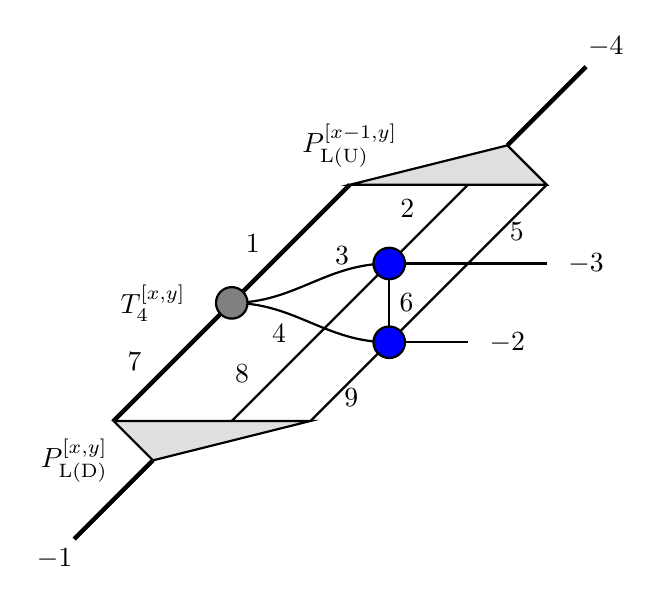
\begin{tikzpicture}[]

		% contant definitions
		\def\tensorSize{0.2}

		% tensor network contraction
		\begin{scope}

			% iPEPS network coordinates
			\coordinate (PN) at (+0.0, +0.5);
			\coordinate (PC) at (+0.0, -0.5);

			% CTMRG network coordinates
			\coordinate (C1) at (-0.5, +1.5);
			\coordinate (T1) at (+1.5, +1.5);
			\coordinate (C2) at (+3.5, +1.5);
			\coordinate (T2) at (+2.0, +0.0);
			\coordinate (C3) at (+0.5, -1.5);
			\coordinate (T3) at (-1.5, -1.5);
			\coordinate (C4) at (-3.5, -1.5);
			\coordinate (T4) at (-2.0, -0.0);

			% projector P_{LU}
			\begin{scope}[shift = {(+1.00, +2.00)}]
				\coordinate (PUL) at (-1.50, -0.50);
				\coordinate (PUM) at (+0.00, -0.50);
				\coordinate (PUR) at (+1.00, -0.50);
				\coordinate (PUU) at (+0.50, +0.00);
				\node[] at (-1.50, -0.00) {$P_\text{L(U)}^{[x - 1, y]}$};
			\end{scope}

			% projector P_{LD}
			\begin{scope}[shift = {(-2.50, -2.00)}]
				\coordinate (PDL) at (-1.00, +0.50);
				\coordinate (PDM) at (+0.50, +0.50);
				\coordinate (PDR) at (+1.50, +0.50);
				\coordinate (PDD) at (-0.50, +0.00);
				\node[] at (-1.50, -0.00) {$P_\text{L(D)}^{[x, y]}$};
			\end{scope}

			% tensor labels
			\node at (-3.0, +0) {$T_4^{[x, y]}$};
			
			% external links
			\draw[thick] (PN) to ($(PN) + (+2.00, +0.00)$) node at ($(PN) + (+2.50, +0.00)$) {$-3$};
			\draw[thick] (PC) to ($(PC) + (+1.00, +0.00)$) node at ($(PC) + (+1.50, +0.00)$) {$-2$};
			\draw[ultra thick] (PDD) to ($(PDD) + (-1.00, -1.00)$) node at ($(PDD) + (-1.25, -1.25)$) {$-1$};
			\draw[ultra thick] (PUU) to ($(PUU) + (+1.00, +1.00)$) node at ($(PUU) + (+1.25, +1.25)$) {$-4$};
			
			% projectors
			\draw[thick, fill = gray!25] (PUL) to (PUR) to (PUU) -- cycle;
			\draw[thick, fill = gray!25] (PDL) to (PDR) to (PDD) -- cycle;

			% internal links
			\draw[ultra thick] (T4) -- (PDL) node[left = 0.25] at ($(T4)!0.5!(PDL)$) {$7$};
			\draw[ultra thick] (T4) -- (PUL) node[left = 0.25] at ($(T4)!0.5!(PUL)$) {$1$};
			\draw[thick] (PN) to [out = 225, in = 45] (PDM) node[left = 0.25] at ($(PN)!0.7!(PDM)$) {$8$};
			\draw[thick] (PUM) to [out = 225, in = 45] (PN) node[left = 0.25] at ($(PUM)!0.3!(PN)$) {$2$};
			\draw[thick] (PC) to [out = 225, in = 45] (PDR) node[right] at ($(PC)!0.7!(PDR)$) {$9$};
			\draw[thick] (PUR) to [out = 225, in = 45] (PC) node[right] at ($(PUR)!0.3!(PC)$) {$5$};
			\draw[thick] (T4) to [out =   0, in = 180] (PC) node[below] at ($(T4)!0.3!(PC)$) {$4$};
			\draw[thick] (T4) to [out =  0, in = 180] (PN) node[above] at ($(T4)!0.7!(PN)$) {$3$};
			\draw[thick] (PN) -- (PC) node [midway, right] {$6$};

			% CTMRG tensors
			\foreach \tensor in {T4} {
				\draw[thick,black,fill = gray] (\tensor) circle (\tensorSize);
			}

			% iPEPS tensors
			\foreach \tensor in {PN, PC} {
				\draw[thick,black,fill = blue] (\tensor) circle (\tensorSize);
			}
			
		\end{scope}

	\end{tikzpicture}

\end{document}
%%% Local Variables:
%%% mode: latex
%%% TeX-master: t
%%% End:
